\documentclass[12pt]{article}
\usepackage{tikz}
\begin{document}
	\begin{tikzpicture}[xscale=2,yscale=1]%%scale=0,8;2
		\clip(-.5,-.5)--(2,0)--(2,.5)--(-.5,.5)--cycle;
		\draw (0,0)--(1,0)--(1,1) (0,0)--(-1,-1);

		\draw (0,0)--(30:1)--(60:1)--cycle; % cycle: vissza az elejére
	\end{tikzpicture}
		
	\begin{tikzpicture}
		\draw[xshift=2cm](-2,0)--+(1,0)--+(0,1);
		\draw [rotate=45](2,0)--++(1,0)--++(0,1);
	\end{tikzpicture}
	\\
	\\
	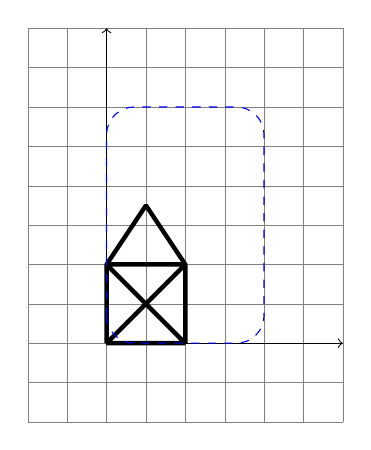
\begin{tikzpicture}
		\draw[help lines, ultra thin, step=.5](-1,-1)grid(3,4);
		\draw[scale=.5, ultra thick,line cap=rectangle,line join=bevel](0,0)--(0,2)--(1,3.5)--(2,2)--(2,0)--(0,2)--(2,2)--(0,0)--(2,0);
		\draw[<->](3,0)--(0,0)--(0,4);
		\draw[blue,dashed,rounded corners=10pt](0,0)rectangle(2,3);
	\end{tikzpicture}

	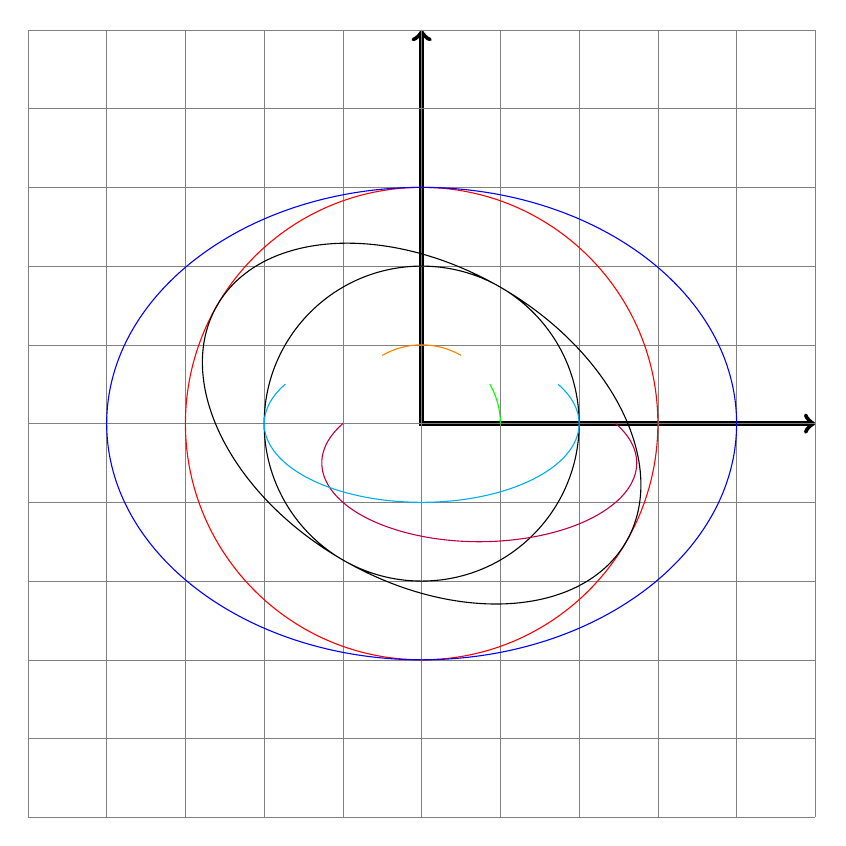
\begin{tikzpicture}
		\draw[<->,ultra thick](5,0)--(0,0)--(0,5);
		\draw[help lines](-5,-5)grid(5,5);
		\draw[red](0,0)circle(3cm);
		\draw(0,0)circle[radius=2cm] circle[x radius =3cm, y radius = 2cm, rotate = -30];
		\draw[blue](0,0)circle(4cm and 3cm);
		\draw[green](1,0)arc(0:30:1cm);
		\draw[orange](60:1) arc(60:120:1cm);
		\draw[purple](-1,0)arc(150:390:2cm and 1cm);
		\draw[cyan](-2,0)arc(180:150:2cm and 1cm)(-2,0) arc(180:390:2cm and 1cm);
	\end{tikzpicture}
	\\ \\ \\ \\
	\tikz{
		\draw[<->](3,0)--(0,0)--(0,3);
		\draw(0,0)--(2,0);
		\draw[blue](0,0)to[bend right](2,0);
		\draw(2,2) to[bend right] (2,0);
		\draw[purple](0,0) to[out=30,in=150](2,0);%vektorok szöggel, és ezek érintőt összeköti
		\draw[red](0,0)..controls(-1,2)..(0,3);
		\draw[cyan](0,0)..controls(-1,2)and(-2,1)..(0,3);
	}

	\tikz{
		\filldraw[draw=red,fill=orange!20!pink](0,0)circle(1cm);
		\filldraw[draw=blue,opacity=0.7](1,1)circle(1cm);
		\shade[top color=green,bottom color=orange,rotate=45](2,-2)rectangle++(2,2);
		%vagy \path a \filldraw helyett		
	}
	\tikz{\fill(1,0) arc (0:90:1cm);}
	\tikz{\fill(0,0)--(1,0) arc (0:90:1cm)--(0,0);}
	
	\tikz{
		\draw[help lines](-2,-2)grid(3,3);
		\draw(0,0)node[below,draw,circle,fill=blue!20,text=purple,outer sep=5pt,inner sep=5pt, thick, dashed]{A}--(1,1)node[pos=0.5,below right]{c}node[above right]{B}--(-1,1)node[above left]{C}--cycle;
		\draw[|-|](0,0)--(3,0)node[pos=.5,below,align=center]{\tiny 3cm\\második sor};
		\draw [->](-1,-1)to[bend right]node[pos=.7,sloped,below]{70\%}(3,-1);
	}
	\tikz{\draw(0,0)node[draw,circle]{A}--(2,0)node[draw,circle]{B};
	\node[draw,circle](a) at (0,-1){A};
	\node[draw,circle](b) at (2,-1){B};
	\draw[->](a)--(b);
	\node[draw,circle](c) at (0,-3){C};
	\draw (a) to[bend right] (c)(a) to[bend left] (c);
	}
	
	\tikz{
		\node[draw,rectangle,ultra thick,inner sep=12pt,align=left](a) at (0,0){print('hello world!')\\// I/O művelet};
		\node[draw,rectangle,rounded corners=14pt,ultra thick, inner sep=12pt](b) at (0,2.5){START};
		\node[draw,rectangle,rounded corners=14pt,ultra thick, inner sep=12pt](c) at (0,-2.5){STOP};
		\draw[->,ultra thick](b)--(a);
		\draw[->,ultra thick](a)--(c);
	}
\end{document}
